%!TEX program = xelatex
\documentclass[a4paper,UTF8]{ctexart}
\usepackage[unicode=true,colorlinks,urlcolor=blue,linkcolor=blue,bookmarksnumbered=true]{hyperref}
\usepackage{latexsym,amssymb,amsmath,amsbsy,amsopn,amstext,amsthm,amsxtra,color,multicol,bm,calc,ifpdf}
\usepackage{graphicx}
\usepackage{diagbox}   % 绘制表格斜线
\usepackage{enumerate}
\usepackage{epstopdf}
\usepackage{fancyhdr}
\usepackage{subfigure}
\usepackage{listings}
\usepackage{multirow}
\usepackage{makeidx}
\usepackage{xcolor} 
\usepackage{algorithm}    % format of the algorithm
\usepackage{algorithmic}    % format of the algorithm
\usepackage{fontspec}                            % 建立索引宏包
\graphicspath{{figures/}}  % 设置图片搜索路径
\theoremstyle{plain} \newtheorem{theorem}{定理}[section]
\theoremstyle{plain} \newtheorem{definition}{定义}[section]
\theoremstyle{plain} \newtheorem{lemma}{引理}[section]
\theoremstyle{plain} \newtheorem{proposition}{命题}[section]
\theoremstyle{plain} \newtheorem{example}{例}[section]
\theoremstyle{plain} \newtheorem{remark}{注}[section]
\theoremstyle{plain} \newtheorem{corollary}{推论}[section]
\newfontfamily\courier{Courier New}
\lstset{linewidth=1.1\textwidth,
        numbers=left, %设置行号位置 
        basicstyle=\small\courier,
        numberstyle=\tiny\courier, %设置行号大小  
        keywordstyle=\color{blue}\courier, %设置关键字颜色  
        %identifierstyle=\bf,
        commentstyle=\it\color[cmyk]{1,0,1,0}\courier, %设置注释颜色 
        stringstyle=\it\color[RGB]{128,0,0}\courier,
        %framexleftmargin=10mm,
        frame=single, %设置边框格式  
        backgroundcolor=\color[RGB]{245,245,244},
        %escapeinside=``, %逃逸字符(1左面的键),用于显示中文  
        breaklines, %自动折行  
        extendedchars=false, %解决代码跨页时,章节标题,页眉等汉字不显示的问题  
        xleftmargin=2em,xrightmargin=2em, aboveskip=1em, %设置边距  
        tabsize=4, %设置tab空格数  
        showspaces=false %不显示空格  
        basicstyle=\small\courier
       }  
\newenvironment{mysolution}{{\color{blue} 解}: }{{\color{magenta}\qed}}
\newcommand\diff{\,{\mathrm d}} %定义微分d
\newcommand{\p}[3]{\frac{\partial^{#1}#2}{\partial{#3}^{#1}}}  %定义求偏导算子
\newcommand{\ucite}[1]{\textsuperscript{\cite{#1}}}  %参考文献引用:上标用\ucite{ },文中用\cite{ }

\begin{document}
\title{

\includegraphics[width=0.65\textwidth]{onepiece.pdf}\\
\vspace{2em}
\textbf{CNN 学习笔记}}
\author{\emph{李向阳} \quad {\color{blue} d1142845997@gmail.com} }
\date{}


\maketitle
\thispagestyle{empty}

\newpage


\tableofcontents

\newpage

\section{引入}
卷积神经网络(Convolutional Neural Network, CNN)也是一个很重要的分类器, 只不过在图像分类中用的比较多, 我目前对图像处理的知识也了解不多, 所以没有太研究它, 不过 CNN 确实太重要而且强大了, 因此还是有必要稍微学习一下. 之前已经介绍过前向神经网络以及反向传播算法了, 所以我会尽量保持体系的一致性, 不去引入太多的图像背景.


\section{CNN 基本模型}
下面大致介绍一下 CNN 模型, 主要以一个实际的编程例子为载体, 即 UFLDL 的 CNN 练习: \url{http://ufldl.stanford.edu/tutorial/supervised/ExerciseConvolutionalNeuralNetwork/}, 这个小例子采用的是熟悉的 MNIST 数据集, 用的是 Matlab 编程, 其程序解答可参考 tornadomeet 的博客: \url{http://www.cnblogs.com/tornadomeet/p/3468450.html}, 这个人的系列博客也很不错. 

这个例子只用了一个卷积层, 一个池化(pooling)层, 和一个 softmax 层(全连接层), 是比较简单清晰的. 其中卷积层有$20$个卷积核, 每个卷积核的大小为$9 \times 9$, pooling 区域大小为$2 \times 2$. 整个模型的基本框架介绍参考的是博客: \url{http://blog.csdn.net/stdcoutzyx/article/details/41596663}.

\subsection{图像卷积和池化}
要理解 CNN 模型, 了解一些基本的图像处理知识是必须的, 关于图像卷积及如何运算, 可以参考 zouxy09 的博客: \url{http://blog.csdn.net/zouxy09/article/details/49080029}. 关于池化, 可参考 UFLDL 上的介绍, 即 \url{http://deeplearning.stanford.edu/wiki/index.php/%E6%B1%A0%E5%8C%96}.

图像的卷积计算如下图 \ref{cal-convole}.
\begin{figure}[!htb]
	\centering
	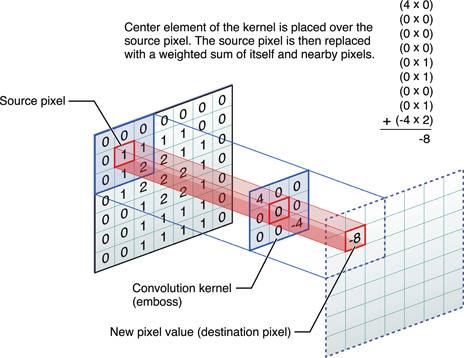
\includegraphics[width=0.65\textwidth]{kernel_convolution.jpg}
	\caption{卷积的计算}
	\label{cal-convole}
\end{figure}

对于一个$28 \times 28$的图像, 和一个$9 \times 9$的卷积核(kernel, 也称为滤子、过滤器, filter)作卷积, 得到的图像大小是$28 - 9 + 1 = 20$, 即新图像的大小是$20 \times 20$, 可参考 UFLDL: \url{http://deeplearning.stanford.edu/wiki/index.php/%E5%8D%B7%E7%A7%AF%E7%89%B9%E5%BE%81%E6%8F%90%E5%8F%96}.

事实上, 这里我们是没有考虑边缘(border), 或者说把边缘去掉了, 如下图 \ref{noborder}.
\begin{figure}[!htb]
	\centering
	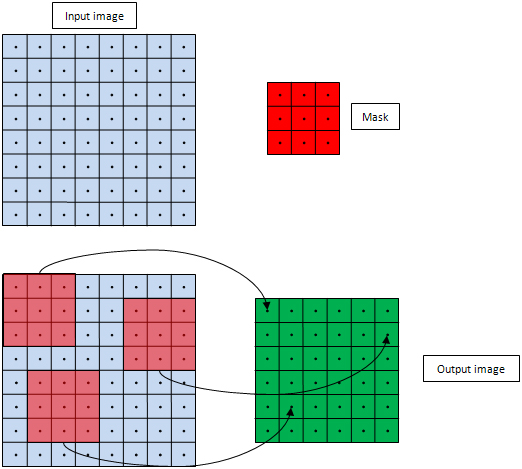
\includegraphics[width=0.65\textwidth]{convolution_trans.jpeg}
	\caption{无边界卷积示意图}
	\label{noborder}
\end{figure}

当然, 也可以对边缘进行计算(如何计算可参考其他资料), 这样得到的图像大小不变, 如下图 \ref{withborder}.
\begin{figure}[!htb]
 	\centering
 	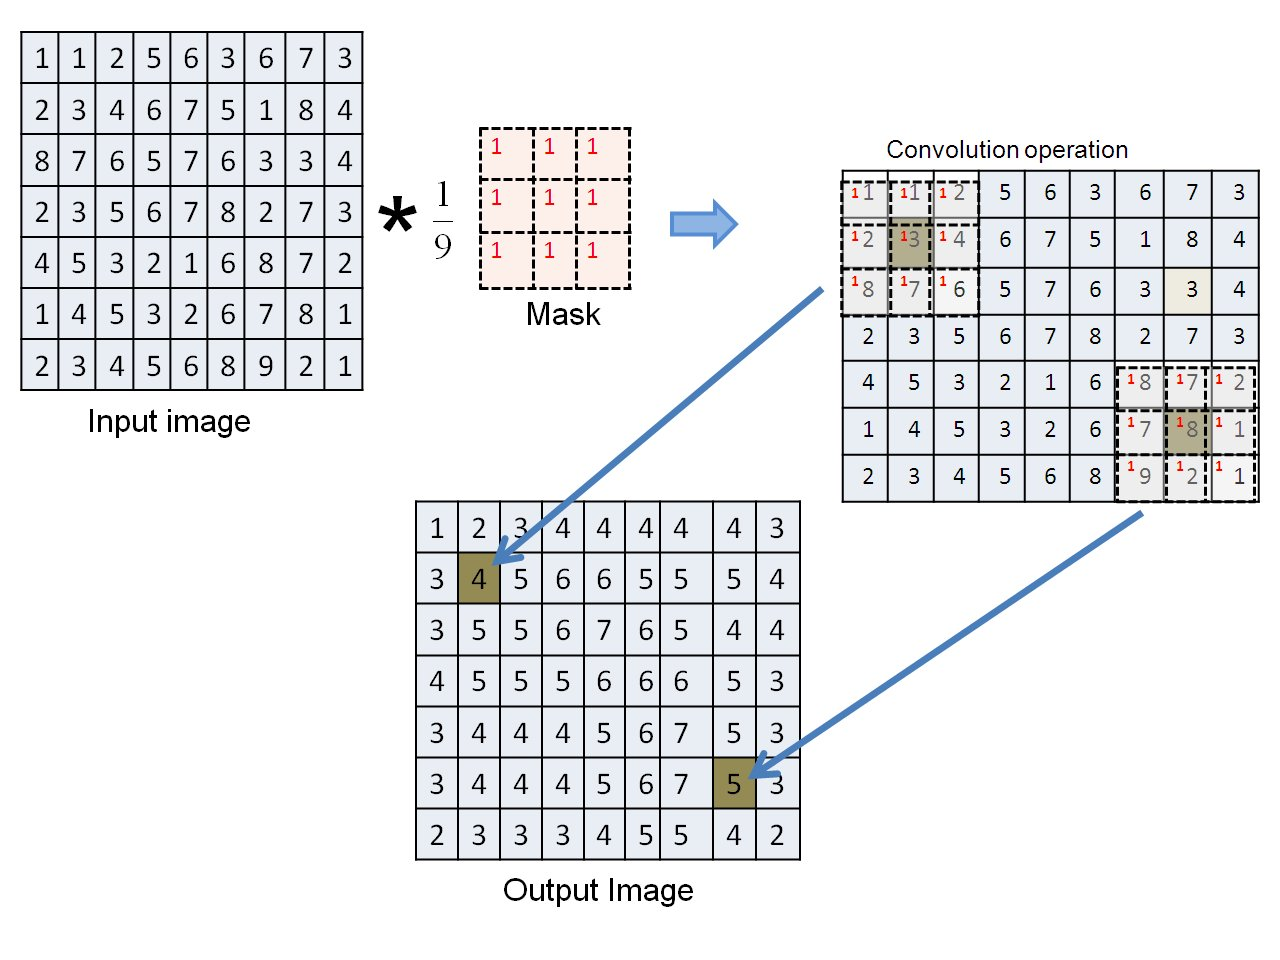
\includegraphics[width=0.65\textwidth]{convolution_fig.jpg}
 	\caption{有边界卷积示意图}
 	\label{withborder}
 \end{figure} 

\subsection{局部感知}
在前向神经网络中, 层之间的神经元是全连接的, 这样的话模型参数太多. 于是, 我们可以让神经元之间局部连接. 在例子中, MNIST 的每个图像都是$28 \times 28$的, 也就是说输入层有$784$个神经元, 假设隐藏层里每个神经元只和输入层的$9 \times 9 = 81$个神经元相连接(其实是选用了$9 \times 9$大小的卷积核), 隐藏层共有$400$个神经元, 其实这$400$个神经元里的像素值构成了一个$20 \times 20$的图像.

计算隐藏层(卷积层)中每个神经元的值时, 需要$9 \times 9$个权重参数(暂不考虑偏置项), 这样的话共需要$400 \times 9 \times 9$个参数.
\begin{figure}[!htb]
    \centering
    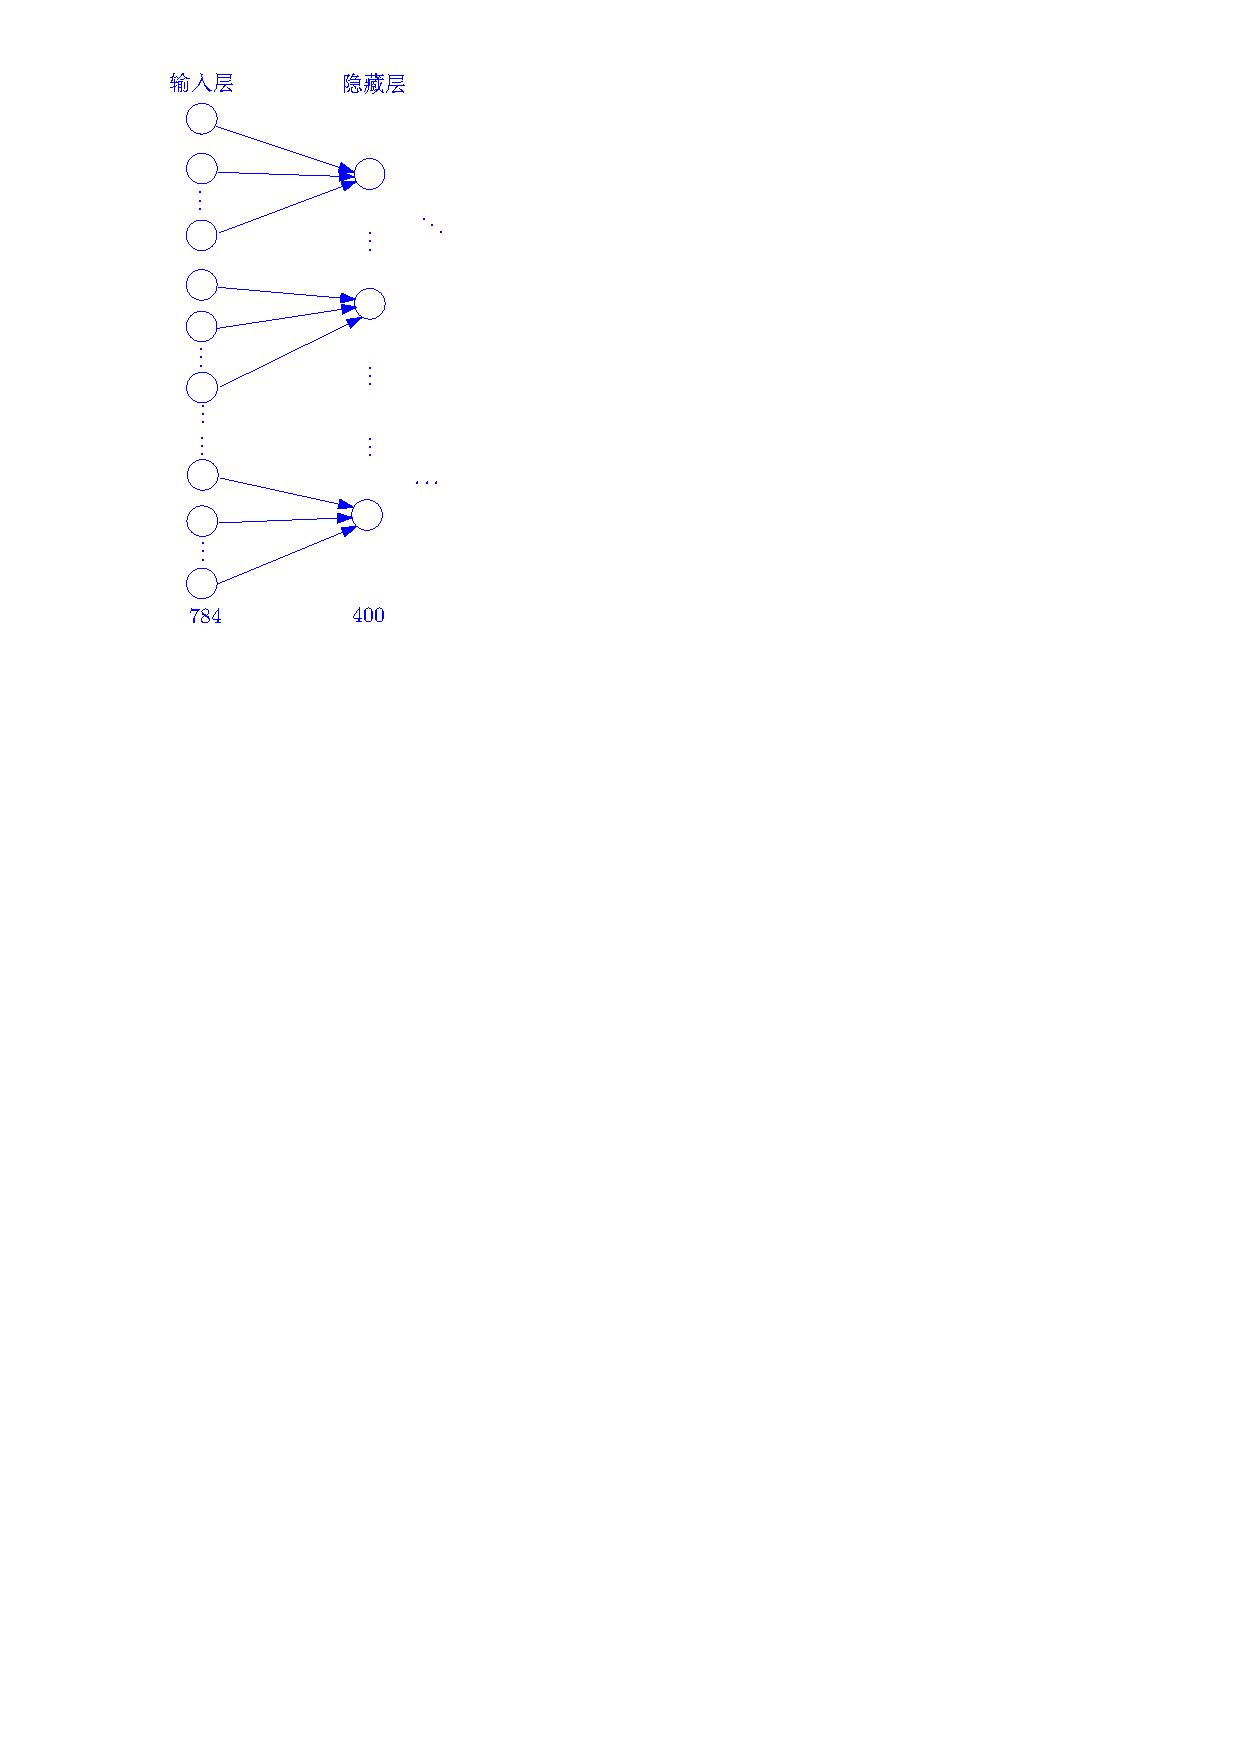
\includegraphics[width=0.35\textwidth]{some_neru.pdf}
    \caption{局部连接示意图}
    \label{some-neru}
\end{figure}

图 \ref{some-neru} 是一个示意图, 当然, 其实输入层的每个神经元不是完全只利用一次的, 只不过为了清晰, 我把它们画开了.

\subsection{权值共享}
假如计算卷积层中每个神经元时, 需要的$9 \times 9$个权重参数是完全一样的, 这就是权值共享, 那么实际计算卷积层仅需要$9 \times 9$个参数, 参数的数量大大减少了.

\subsection{多卷积核}
上面是只有一个卷积核, 显然特征提取不充分, 于是我们可以添加多个卷积核, 比如例子中是$20$个卷积核. 前面提到, 一个卷积核(权值共享)对原图像作用得到$400$个像素值, 相当于生成了一幅$20 \times 20$的图像, 现在有$20$个不同的卷积核, 相当于生成了$20$幅不同的图像, 这可以看做是原图像的$20$个不同的通道. 因此, 卷积层实际含有的神经元个数为$20 \times 400$, 不过参数个数只有$20 \times 9 \times 9$个(算上偏置参数的话, 再加个$20 \times 1$即可).

回到我们的例子, 用一个卷积核得到了$400$个神经元, 相当于是一个$20 \times 20$的图像, 此时维数较高, 我们通过采样(sampling)或者说池化(pooling)进行聚合, 即将图像上的一个区域用该区域上的某个特定特征的平均值(或最大值)来替代, 也称为平均池化(或最大池化). 我们的例子中, 池化区域的大小是$2 \times 2$, 如此一来, $400$个像素值就变成了$100$个像素值, 相当于图像由$20 \times 20$变为了$10 \times 10$. 由于有$20$个卷积核, 因此池化层实际含有的神经元个数为$20 \times 100$. 接下来我们将池化层和最后的输出层(含有$10$个输出单元)之间进行全连接(softmax 连接), 参数个数为$20 \times 100 \times 10$(算上偏置参数的话, 再加个$1 \times 10$即可). 这样, 我们例子中的卷积神经网络就完成了. 算上偏置参数的话, 模型参数总共有$20 \times 9 \times 9 + 20 + 20 \times 100 \times 10 + 10 = 21650$个.

以上是为了体系的一致性, 主要采用神经元的方式叙述的, 如果直接用图像表示的话, 大致过程如下图 \ref{convole}.
\begin{figure}[!htb]
	\centering
	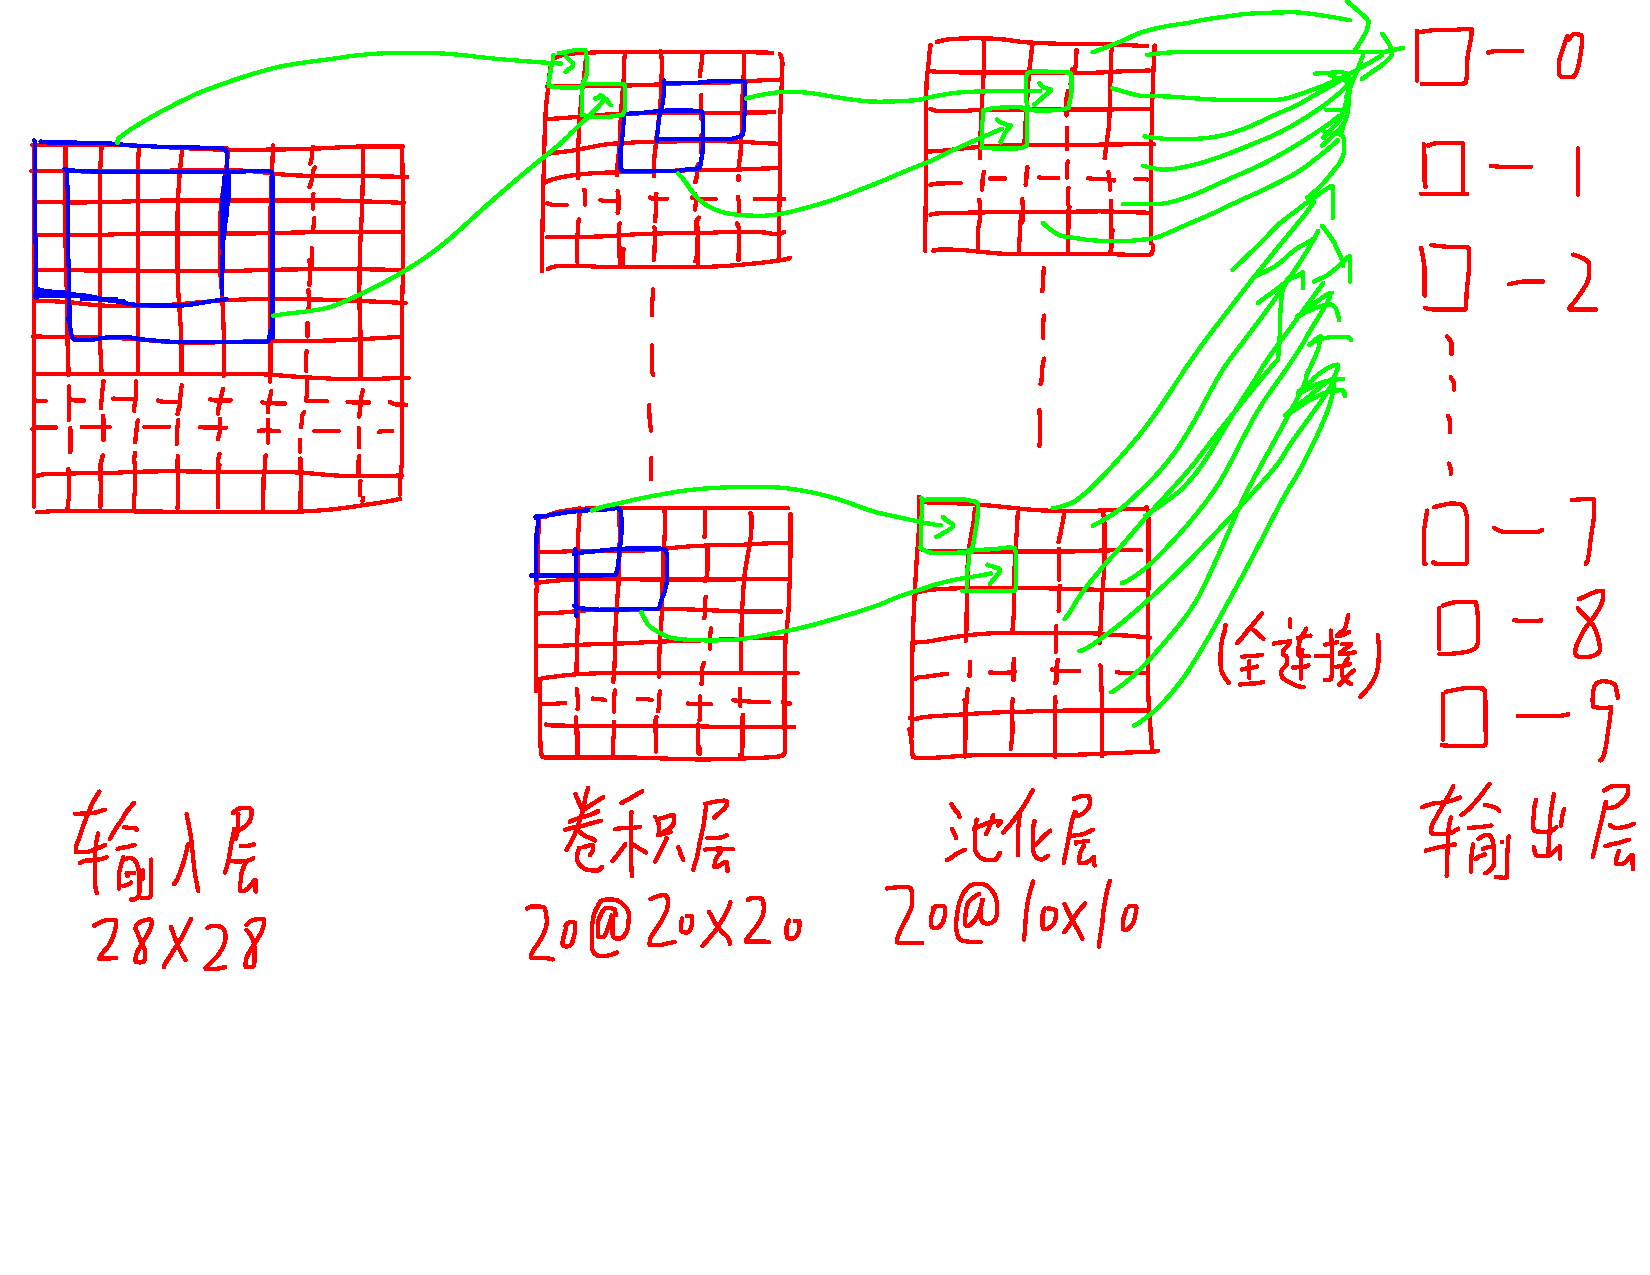
\includegraphics[width=0.85\textwidth]{convole.pdf}
	\caption{CNN 示意图}
	\label{convole}
\end{figure}

当然, 对于更复杂的问题, 我们可能会构造更多的卷积层. 比如经典的 LeNet5, 其网络结构说明可参考: \url{http://www.cnblogs.com/tornadomeet/archive/2013/05/05/3061457.html}.

\subsection{Dropout}
CNN 也会存在过拟合问题, 而 Dropout 有助于缓解这一问题. Dropout 层将随机丢弃(drop out)该层中一些权值参数, 即在前向传播过程中将这些激活参数集设置为 0, 相当于随机删除一些节点神经元和相应的边, 有种类似于决策树中剪枝的思想, 这可以减轻模型的复杂度, 一定程度上避免过拟合.



\section{反向传播推导}
上面我们是用一个简单的例子来说明了卷积神经网络, 其中为了简化, 很多地方也表述的不够严谨, 但有助于理解. CNN 模型的参数很多, 那么如何求得这些参数呢? 

其实, 同前向神经网络一样, 模型参数的学习也是反向传播算法. 关于其具体推导, 可以参考 tornadomeet 的博客: \url{http://www.cnblogs.com/tornadomeet/p/3468450.html}, 当然也可以看相关论文或者 notes. 由于 CNN 不仅有 softmax 全连接层, 还有卷积层和池化层, 卷积层的具体卷积方式也不同, 因此 CNN 的反向传播还是很复杂的.







\section{总结}
\subsection{参考资料}
\begin{enumerate}[(1)]
\item tornadomeet 的博客: \url{http://www.cnblogs.com/tornadomeet/p/3468450.html}, 里面有 CNN 的反向传播推导和本次例子的 Matlab 代码. 他的系列博客也都还不错.

\item UFLDL 上关于 CNN 的练习: \url{http://ufldl.stanford.edu/tutorial/supervised/ExerciseConvolutionalNeuralNetwork/}.


\end{enumerate}





\newpage

\section*{附录}








\end{document}